\chapter{Appendix for {\BIAREL}}
\label{AppB}

We use some abbreviations throughout in the appendix, "TS" for "To show", RTS stands
for ``remains to show", STS stands for ``suffices to
show".  "IH" for induction hypothesis, "IH2" for induction hypothesis on the second goal, which is usually when simultaneously proving multiple goals in a lemma, similar for "IH3", "IH4", and so on.

\section{\relstlc}
\label{appendixb:relstlc}
 \subsection{Syntax of \relstlc}
 \label{appendixb:relstlc-syntax}
  \input{chapters/birelcost/RSTLC/relstlc_figures}
  \clearpage
  \subsection{Metatheory of \relstlc}
  \label{appendixb:relstlc_lemma}
 \input{chapters/birelcost/RSTLC/relstlc_lemmas} 
  \clearpage

\section{\relref}
  \subsection{Syntax of \relref}
  \label{appendixb:relref_syntax}
  \input{chapters/birelcost/RSTLC/relref_figures}
  \clearpage
  \subsection{Metatheory of \relref}
   \label{appendixb:relref_lemma}
  \input{chapters/birelcost/RSTLC/relref_lemmas}
  \clearpage
  
  \section{\relinf}
\subsection{Syntax of \relinf}
 \label{appendixb:relinf_syntax}
   \input{chapters/birelcost/RSTLC/relinf_figures}
  \clearpage
  \subsection{Metatheory of \relinf}
   \label{appendixb:relinf_lemma}
   \input{chapters/birelcost/RSTLC/relinf_lemmas}
   \clearpage
   
\section{\relinfref}
 \subsection{Syntax of \relinfref}
  \label{appendixb:relinfref_syntax}
 \input{chapters/birelcost/RSTLC/relinfref_figures}
 \clearpage
 \subsection{Metatheory of \relinfref}
  \label{appendixb:relinfref_lemma}
  We also use the name RelInfRef for {\relinfref}.
 \input{chapters/birelcost/RSTLC/relinfref_lemmas}   
  \clearpage
  
\section{\Relcost}
\wq{The content of this section is from the Ph.D. thesis of Ezgi Cicek~\citet{cicek2018:thesis}.}
% \begin{itemize}
% \item The constrained type $\tcimpl{C}{\tau}$, which is eliminated with
%   the ``$\ecelim e$'' construct.
% \item The type $\achange\,\grt$ is generalized to
%   $\tch{\grt_1}{\grt_2}$ (like in {\Relcost}'s appendix), allowing us to
%   relate two expressions of two different unary types $\grt_1$ and
%   $\grt_2$, respectively. As a result of this change, \textbf{switch}
%   rule, \textbf{$\to \wexec$} subtyping rule, and some of the
%   asynchronous rules are also generalized.%  The advantage of this
%   % generalization is useful for the $\kw{2Dcount}$ example, explained
%   % in depth in Section \ref{sec:examples}.

% \end{itemize}

It first presents {\Relcost}'s syntax, typing and subtyping rules. Then,
it introduces {\relcostmin} and the embedding of {\Relcost} into
{\relcostmin}. Finally, the bidirectional system {\birelcost} is
introduced. 

\clearpage

 
The syntax is shown as follows,
\[
\begin{array}{llll}
\mbox{Arithmetic Operators} 
& \oplus_a & ::= & + ~|~ - ~|~ \times 
%
~|~ \div ~|~ \max ~|~ \min\\  
% \mbox{Unary Operators} 
% & \oplus_a & ::= & + ~|~ - ~|~ \times 
% %
% ~|~ \div \\  
\mbox{Boolean Operators} 
& \oplus_b & ::= & \lor ~|~ \land
\\
%
\mbox{Relational Operators} 
& \sim & ::= & < ~|~ \leq ~|~ == 
\\  
%
\mbox{Label} 
& l & \in & \mathbb{N} \cup \{\lin, \lex\} 
\\ 
%
\mbox{Arithmetic Expression} 
& \aexpr & ::= & 
n ~|~ {x} ~|~ \aexpr \oplus_a \aexpr  
% \\
% &  &  & 
 ~|~ \elog \aexpr  ~|~ \esign \aexpr
\\
%
\mbox{Boolean Expression} & \bexpr & ::= & 
%
\etrue ~|~ \efalse  ~|~ \neg \bexpr
 ~|~ \bexpr \oplus_b \bexpr
%
~|~ \aexpr \sim \aexpr 
\\
%
\mbox{Expression} & \expr & ::= & v ~|~ \aexpr ~|~ \bexpr ~|~ [\expr, \dots, \expr]
\\  
%
\mbox{Value} 
& v & ::= & { n ~|~ \etrue ~|~ \efalse ~|~ [] ~|~ [v, \dots, v]}  
\\
%
\highlight{\mbox{Query Expression}  }
& {\qexpr} & ::= 
& \highlight{ \qval ~|~ \aexpr ~|~ \qexpr \oplus_a \qexpr ~|~ \chi[\aexpr]}
\\
%
\highlight{\mbox{Query Value} }& \qval & ::= 
& \highlight{n ~|~ \chi[n] ~|~ \qval \oplus_a  \qval ~|~ n \oplus_a  \chi[n]
    ~|~ \chi[n] \oplus_a  n}
    \\
% &&& \text{\mg{I don’t think this is what I want. Isn’t $\chi[n+1]$ a query value?}}\\
% &&& \text{\mg{What about $\chi[i] + \chi[i] + \chi[i]$? They are not in the grammar}}
% \\
% &&& \text{\jl{ $\chi[i] + \chi[i] + \chi[i]$ and $\chi[n+1]$ are both expressions, they will be evaluated to a value 
% }}
% \\%
\mbox{Labeled Command} 
& {c} & ::= &   [\assign {{x}}{ {\expr}}]^{l} ~|~  \highlight{[\assign {{x} } {{\query(\qexpr)}}]^{l}}
~|~ {\ewhile [ \bexpr ]^{l} \edo {c} }
\\
&&&
~|~ {c};{c}  
~|~ \eif([\bexpr]{}^l , {c}, {c}) 
~|~ [\eskip]^l
\\ 
\mbox{Event} 
& \event & ::= & 
    ({x}, l, v, \bullet) ~|~ ({x}, l, v, \qval)  ~~~~~~~~~~~ \mbox{Assignment Event} \\
&&& ~|~(\bexpr, l, v, \bullet)   ~~~~~~~~~~~~~~~~~~~~~~~~~~~~~~~~~~ \mbox{Testing Event}
\\
\mbox{Trace} & \trace
& ::= & [] ~|~ \trace :: \event
\\
\end{array}
\]
% \[
% \begin{array}{llll}
% \mbox{Arithmetic Operators} 
% & \oplus_a & ::= & + ~|~ - ~|~ \times 
% %
% ~|~ \div ~|~ \max ~|~ \min\\  
% % ~|~ \div \\  
% \mbox{Boolean Operators} 
% & \oplus_b & ::= & \lor ~|~ \land
% \\
% %
% \mbox{Relational Operators} 
% & \sim & ::= & < ~|~ \leq ~|~ == 
% \\  
% %
% \mbox{Arithmetic Expression} 
% & \aexpr & ::= & 
% n ~|~ {x} ~|~ \aexpr \oplus_a \aexpr  
%  ~|~ \elog \aexpr  ~|~ \esign \aexpr
% \\
% %
% \mbox{Boolean Expression} & \bexpr & ::= & 
% %
% \etrue ~|~ \efalse  ~|~ \neg \bexpr
%  ~|~ \bexpr \oplus_b \bexpr
% %
% ~|~ \aexpr \sim \aexpr 
% \\
% %
% \mbox{Expression} & \expr & ::= & v ~|~ \aexpr ~|~ \bexpr ~|~ [\expr, \dots, \expr] ~|~ \highlight{\fname}
% \\  
% %
% \mbox{Value} 
% & v & ::= & { n ~|~ \etrue ~|~ \efalse ~|~ [] ~|~ [v, \dots, v]}  
% \\ 
% &&&
% \highlight
% {
% ~|~ (x_0, x_1, \ldots, x_n) := c
% }
% \\
% %
% \highlight{\mbox{Query Expression}} 
% & {\qexpr} & ::= 
% & \highlight{ \qval ~|~ \aexpr ~|~ \qexpr \oplus_a \qexpr ~|~ \chi[\aexpr]} 
% \\
% %
% \mbox{Query Value} & \qval & ::= 
% & \highlight{n ~|~ \chi[n] ~|~ \qval \oplus_a  \qval ~|~ n \oplus_a  \chi[n]
%     ~|~ \chi[n] \oplus_a  n}
% \\
% % \\%
% \mbox{Label} 
% & l & ::= & (n \in \mathbb{N} \cup \{\lin, \lex\}) ~|~ (l, n)
% \\ 
% %
% \mbox{Labeled Command} 
% & {c} & ::= &  
% \clabel{\assign{x}{\expr}}^l 
% ~|~ \clabel{\assign{x}{\query(\qexpr)}}^l
% ~|~  \clabel{\eskip}^l
% ~|~ \ewhile \clabel{\bexpr}^{l} \edo {c}
% ~|~ \eif(\clabel{\bexpr}^{l} , {c}, {c}) 
% \\ 
% &&&
% \highlight
% {
% ~|~ \clabel{\efun}^l: \fname (x_0, x_1, \ldots, x_n) := c
% ~|~ \clabel{\assign{x}{\ecall(x, e_1, \ldots, e_n)}}^l
% }
% ~|~ {c};{c}  
% \\ 
% % \\
% \mbox{Event} 
% & \event & ::= & 
%     ({x}, l, v, \bullet) ~|~ ({x}, l, v, \qval) ~|~ (\fname, l, v, \qval)  ~~~~~~~~~~~ \mbox{Assignment Event} \\
% &&& ~|~(\bexpr, l, v, \bullet)   ~~~~~~~~~~~~~~~~~~~~~~~~~~~~~~~~~~ \mbox{Testing Event}
% \\
% % &&& \text{\mg{I think it would be better to use quadruples for events, where the}}\\
% % &&& \text{\mg{first element is either a variable or a boolean expression and }}\\
% % &&& \text{\mg{the last is either a query value or some default value $\bullet$}}\\
% %
% % \mbox{Trace} & \trace
% % & ::= & \cdot | \trace \cdot \event | \trace \tracecat \trace 
% % \\
% %
% % \mbox{Trace} & \trace
% % & ::= & [] ~|~ \event:: \trace ~|~ \trace \tracecat \trace  \\
% \mbox{Trace} & \trace
% & ::= & [] ~|~ \trace :: \event\\
% % &&& \text{\mg{I don't understand why you need both :: and ++ as constructors.}}\\
% % &&& \text{\jl{Because append is to the left but we are adding element to the left in the OS}}\\
% % &&& \text{\jl{I was too sticky to the convention, it is a good idea to append to the left and just use $::$}}
% % %
% % \mbox{Event Signature} & \sig
% % & ::= & (x, l, n) | (x, l, n, \query) | (b, l, n)
% % \\
% % %
% \end{array}
% \]
For clarity, the following notations are used to represent the set of corresponding terms:
\[
\begin{array}{lll}
\mathcal{VAR} & : & \mbox{Set of Variables}  
\\ 
%
\mathcal{VAL} & : & \mbox{Set of Values} 
\\ 
%
\mathcal{QVAL} & : & \mbox{Set of Query Values} 
\\ 
%
\cdom & : & \mbox{Set of Commands} 
\\ 
%
\mathcal{LV} & : & \mbox{Set of Labeled Variables}
\\
%
\eventset  & : & \mbox{Set of Events}  
\\
%
\eventset^{\asn}  & : & \mbox{Set of Assignment Events}  
\\
%
\eventset^{\test}  & : & \mbox{Set of Testing Events}  
\\
%
\ldom  & : & \mbox{Set of Labels}  
\\
%%
\mathcal{VAL}  & : & \mbox{Set of Labeled Variables}  
\\
%%
\dbdom  & : & \mbox{{Set of Databases}} 
\\
%
{\mathcal{T}} & : & \mbox{Set of Traces}
\\
%
% \qdom = {[-1,1]} & : & \mbox{{Domain of Query Results}}\\
\qdom & : & \mbox{{Domain of Query Results}}\\
% &&\text{\mg{I don't think you need to hard code [-1,1] here}}\\
\end{array}
\]
\paragraph*{Standard Expression}
The expressions are either the standard one or the extended one.
A standard expression is
% can be 
either a standard arithmetic expression or a boolean expression, or a list of expressions.
An arithmetic expression can be a constant $n$ denoting integer, a variable $x$ from some countable set $\mathcal{VAR}$, binary operation $\oplus_a$ such as addition, product, subtraction, etc, over arithmetic expressions, and also log and sign operation. 
%
A boolean expression can be either {\tt true} or {\tt false}, basic boolean connectives such as logical negation, logical and and or denoted by $\oplus_b$, and basic comparison $sym$ between arithmetic expressions, e.g., $\leq,=,<,$ etc.
Additionally, I also introduce list in expression.
Our language supports primitives for queries, 
where a specific query is specified by a query expression $\qexpr$. 
A query expression contains the necessary information for a query request, for example, 
$\chi[\aexpr]$ represents the values at a certain index $\aexpr$ in a row $\chi$ of the database. 
Query expressions combine access to the database with other expressions, 
for example, $\chi[3] + 5$ represents a query which asks the value from the column 3 of each database raw $\chi$, adds 5 to each of these values, 
and then computes the average of these values.
\paragraph*{Query Expression}
The key extension is
%  language supports 
the primitive for queries, where a specific query is specified by a query expression $\qexpr$. 
A query expression contains the necessary information for a query request, 
for example, $\chi[\qexpr]$ represents the values at a certain index $\qexpr$ in a row $\chi$ of the database. 
When this expression is encapsulated by the symbol $\query$,
 $ \query(\chi[\qexpr]) $ computes the average value at certain index over each row of the database as follows,
 \[
  \query(\chi[\qexpr]) = \frac{1}{n}\sum\limits_{i = 0}^{n}\chi_i[\qexpr]
  \]
Query expressions combine access to the database with other expressions, 
for example, 
$\chi[3] + 5$ represents a query that asks the value from column 3 of each database raw $\chi$, 
adds 5 to each of these values, and then computes the average of these values as follows, where $n$ is 
data base $\chi$'s number of raw.
%
\[
  \query(\chi[3] + 5) = \frac{1}{n}\sum\limits_{i = 0}^{n}\chi_i[3] + 5
  \]

% the expression also includes the special variable $\chi$ representing a row of the database, and access to values at a certain index in $\chi$, as $\chi[\aexpr]$. Additionally, list over expressions is supported and $[]$ stands for the empty list. The access to elements in the list can be achieved through $x[\aexpr]$ when variable $x$ is referred to a list. The value $v$ now contains the natural number $n$, the boolean primitives $\etrue$ and $\efalse$, the special row $\chi$ and access to it $\chi[v]$, the empty list $[]$ and non-empty list $[v, \dots, v]$.
% 
% Another extension is the inter-procedure call and function definition.
% In the function define command $\clabel{\efun}^l: \fname (x_0, x_1, \ldots, x_n) := c$,
% the function body $c$ is assigned to the function of name $\fname$, $x_1, \ldots, x_n$ is the function
% arguments and the first element $x_0$ in the arguments is the return variable.
% We only support the first-order function definition and function call. 

% %
\paragraph*{Labeled Command}
 A labeled command $c$ is just a command with a label --- I assume that labels are unique, so that they can help to identify uniquely every subexpression. 
%  I have $\eskip$, assignment $\assign{x}{\expr}$, the composition of two commands $c;c$, an if statement $\eif(\bexpr, c, c)$, a while statement  $\ewhile \bexpr \edo {c} $.
 The main novelty of the syntax is the query request command $\assign{x}{\query(\qexpr)}$. 
 For instance, if a data analyst wants to ask a simple linear query which returns the first element of the row, 
 they can simply use the command $ \assign{x}{\query(\chi[1])}$ in their data analysis program.
%  \wq{Shall I distinguish command and labeled command, they are now both $c$. }
%  \jl{I'm not sure, I don't want to programmer to add the label when writing the program. The label is just added by us for analysis. but I'm worried it is too complicate if use two notations for command and labeled command }
%
% \[
% \begin{array}{llll}
% \mbox{Label} 
% & l & \in & \mathbb{N} \cup \{in, ex\} \\
% \mbox{Labeled Commands} 
% & {c} & ::= &   [\assign {{x}}{ {\expr}}]^{l} ~|~  [\assign {{x} } {{\query(\qexpr)}}]^{l}
% ~|~ {\ewhile [ \bexpr ]^{l} \edo {c} }
%  \\
%  &&&
% ~|~ {c};{c}  
% ~|~ \eif([\bexpr]{}^l , {c}, {c}) 
% ~|~ [\eskip]^l 
% \end{array}
% \]
\paragraph*{Labeled Variables}
The labeled variables and assigned variables are set of variables annotated by a label. 
We use  
%$\mathcal{LVAR} = \mathcal{VAR} \times \mathcal{L} $ 
$\mathcal{LV}$ represents the universe of all the labeled variables and 
$\avar_c \in \mathcal{P}(\mathcal{VAR} \times \mathbb{N}) \subset \mathcal{LV}$ and 
$\lvar_c \in \mathcal{P}(\mathcal{VAR} \times \mathcal{L}) \subseteq \mathcal{LV}$,
represents the the set of assigned variables and labeled variables for a labeled command $c$,
defined in Definition~\ref{def:lvar} and \ref{def:avar}.
%
% \\
$FV: \expr \to \mathcal{P}(\mathcal{VAR})$, computes the set of free variables in an expression. To be precise,
$FV(\aexpr)$, $FV(\bexpr)$ and $FV(\qexpr)$ represent the set of free variables in arithmetic
expression $\aexpr$, boolean expression $\bexpr$ and query expression $\qexpr$ respectively.
Labeled variables in $c$ is the set of assigned variables and all the free variables
showing up in $c$ with a default label $in$. 
The free variables
showing up in $c$, which aren't defined before be used, are actually the input variables of this program.
%
%
\begin{defn}[Assigned Variables (
% $\avar_{c} \subseteq \mathcal{VAR} \times \mathbb{N}$ or 
$\avar : \cdom \to \mathcal{P}(\mathcal{VAR} \times \mathbb{N})$)]
% labelled Variables 
% (
% % $\lvar_{c} \subseteq \mathcal{VAR} \times \mathbb{N}$ or 
% $\lvar : \cdom \to \mathcal{P}(\mathcal{VAR} \times \mathcal{L})$
\label{def:avar}
$$ \avar_{c} \triangleq
  \left\{
  \begin{array}{ll}
      \{{x}^l\}                   
      & {c} = [{\assign x e}]^{l} 
      \\
      \{{x}^l\}                   
      & {c} = [{\assign x \query(\qexpr)}]^{l} 
      \\
      \avar_{{c_1}} \cup \avar_{{c_2}}  
      & {c} = {c_1};{c_2}
      \\
      \avar_{{c}} \cup \avar_{{c_2}} 
      & {c} =\eif([\bexpr]^{l}, c_1, c_2) 
      \\
      \avar_{{c}'}
      & {c}   = \ewhile ([\bexpr]^{l}, {c}')
\end{array}
\right.
$$
\end{defn}
%
%
\begin{defn}[labelled Variables 
(
% $\lvar_{c} \subseteq \mathcal{VAR} \times \mathbb{N}$ or 
$\lvar : \cdom \to \mathcal{P}(\mathcal{LV})$]
\label{def:lvar}
$$
  \lvar_{c} \triangleq
  \left\{
  \begin{array}{ll}
      \{{x}^l\} \cup FV(\expr)^{in}                  
      & {c} = [{\assign x e}]^{l} 
      \\
      \{{x}^l\}   \cup FV(\qexpr)^{in}                
      & {c} = [{\assign x \query(\qexpr)}]^{l} 
      \\
      \lvar_{{c_1}} \cup \lvar_{{c_2}}  
      & {c} = {c_1};{c_2}
      \\
      \lvar_{{c}} \cup \lvar_{{c_2}} \cup FV(\bexpr)^{in}
      & {c} =\eif([\bexpr]^{l}, c_1, c_2) 
      \\
      \lvar_{{c}'} \cup FV(\bexpr)^{in}
      & {c}   = \ewhile ([\bexpr]^{l}, {c}')
\end{array}
\right.
$$
\end{defn}
%
%
%
% is a subset of the program's assigned variables, where every variable in this set is assigned by a query in the program.
% \mg{The set of query variables of a program is the set of variables set to the result of a query in the program.}\\
% In the same way, in order to 
\paragraph*{Query Variables}
Distinctively, a key definition for the extension of the query primitives 
is the set of query variables for a program $c$.
This definition is the key point to track the query requests in the Following full-spectrum adaptivity analysis.
% track the I also defined the set of query variables for a program $c$.
It is defined as the set of variables,
which are assigned by the result of a query request in the program formally in Definition~\ref{def:qvar}.
% \mg{In the next definition, why do you call it a vector? It seems that you define it as a set.}\\
% \jl{fixed}\\
%
% \begin{defn}[Query Variables ($\qvar_{c} \subseteq \mathcal{VAR} \times \mathbb{N}$)].
  % \\
\begin{defn}[Query Variables ($\qvar: \cdom \to \mathcal{P}(\mathcal{LV})$)] 
  \label{def:qvar}
Given a program $c$, its query variables 
% \mg{it seems you are missing the $_c$ subscript. Also, this is a minor point but I don't think it is a good idea to use a subscript, cannot you just use $\qvar(c)$.}
$\qvar(c)$ is the set of variables set to the result of a query in the program.
% \jl{fixed}
It is defined as follows:
{
$$
  % \qvar_{{c}} \triangleq
  \qvar(c) \triangleq
  \left\{
  \begin{array}{ll}
      % \{\}                  
      % & {c} = [{\assign x e}]^{(l, w)} 
      % \\
      % \{{x}^l\}                  
      % & {c} = [{\assign x \query(\qexpr)}]^{(l, w)} 
      % \\
      % \qvar_{{c_1}} \cup \qvar_{{c_2}}  
      % & {c} = {c_1};{c_2}
      % \\
      % \qvar_{{c_1}} \cup \qvar_{{c_2}} 
      % & {c} =\eif([\bexpr]^{l}, c_1, c_2) 
      % \\
      % \qvar_{{c}'}
      % & {c}   = \ewhile ([\bexpr]^{l}, {c}')
      \{\}                  
      & {c} = [{\assign x \expr}]^{l} 
      \\
      \{{x}^l\}                  
      & {c} = [{\assign x \query(\qexpr)}]^{l} 
      \\
      \qvar(c_1) \cup \qvar(c_2)  
      & {c} = {c_1};{c_2}
      \\
      \qvar(c_1) \cup \qvar(c_2) 
      & {c} =\eif([\bexpr]^{l}, c_1, c_2) 
      \\
      \qvar(c')
      & {c}   = \ewhile ([\bexpr]^{l}, {c}')
\end{array}
\right.
$$
}
\end{defn}
%
It is easy to see that a program $c$'s query variables is a subset of 
its labeled variables, $\qvar(c) \subseteq \lvar(c)$.
%
% \mg{In this definition as well as in others, I have the impression that you assume that the labelled variables are unique in the program. For example, it would not make sense to assign a query to the same labelled variable over and over. If this is the case, I need to make this very explicit in the paper.}
% \jl{TODO}
%
Every labeled variable in a program is unique, formally as follows with proof in Appendix~\ref{apdx:lemma_sec123}.
\begin{lem}[Uniqueness of the Labeled Variables]
  \label{lem:lvar_unique}
  For every program $c \in \cdom$ and every two labeled variables such that
  $x^i, y^j \in \lvar(c)$, then $x^i \neq y^j$.
  \[
    \forall c \in \cdom, x^i, y^j \in \mathcal{L} \sthat x^i, y^j \in \lvar(c)\implies x^i \neq y^j.
    \]
\end{lem}

\highlight{\paragraph*{Improvements through Examples}
It is expressive in two following aspects.
\begin{itemize}
  \item \textbf{Improvements from Standard While Language}
  \\
  It also extends the standard while language with query requests. 
  The general data analysis program with query requests on data  are supported in this {\tt Query While} language.
  The program can access the database through a special  interface $\chi$ encapsulated by the identifier $\query$ (for example the program below) in the new language.
  \[
    {\assign{x}{20}};
    \assign{y}{\query(\chi[2])};
    \ewhile (x < 100) \edo 
    \{
      \assign{x}{x + 1};
      \assign{y}{\query(\chi[x]*\chi[n])};
      \}\}
    \] 
%
    \item \textbf{Improvements from Previous Works}
  \\
This {\tt Query While} language is also more expressive than the language designed in previous works.
The previous language only supports the data analysis with constant number of loop iterations.
Comparing to it, in the new language design,
the general data analysis program with non-deterministic loop iterations
(for example the program below as shown in Section~\ref{sec:prework-language})
is supported.
\[
  {\assign{x}{20}};
  \assign{y}{40};
  \ewhile (x < y) \edo 
  \{
    \assign{x}{x + 1};
    \assign{y}{y - 2};
    \}\}
  \] 
Previous work does not support data analysis program with user inputs, which is supported in the new language as well.
\end{itemize}
}

% \begin{figure}
%   \centering
%   \[ \begin{array}{@{}l@{~~}l@{~}l@{~}l@{}l}
%        \text{meta~variables} & M & \bnfdef & i,n,m, \cdots \\
%        \text{index~terms} & I,k,t & \bnfdef & \cdots~|~ M \\
%        \text{meta~contexts} & \psi &  \bnfdef & \emptyset~ |~ \psi, M : \sort\\
%        \text{meta~substitutions} & \theta &  \bnfdef & []~ |~ \theta[M \mapsto I]\\
%        \text{constraints} & C &  \bnfdef & \cdots ~ |~ \cforallS{i}{S}{C} ~|~ \cexistsK{i}{S}{C} \\
%        \text{expressions} & e &  \bnfdef & \cdots ~ |~ \eanno{e}{\grt}{k}{t} ~|~ \eannobi{e}{\tau}{t} \\
%      \end{array}\]
%    \caption{Extended {\tnamemin} syntax for {\bitname}}
%  \end{figure}


\input{chapters/birelcost/appendix/types-wf}
\input{chapters/birelcost/appendix/constraint-gen}

%\input{subtyping-rules-defs}
\input{chapters/birelcost/appendix/subtyping-rules}


%\input{typing-rules-defs}
\input{chapters/birelcost/appendix/typing-rules}

% Elaboration
%\input{elaboration-rules-defs} 
\input{chapters/birelcost/appendix/elaboration-rules} 

% RelCost Core System
%\input{type-eq-rules-defs}
\input{chapters/birelcost/appendix/type-eq-rules}
%\input{typing-rules-min-defs}
\input{chapters/birelcost/appendix/typing-rules-min}

\clearpage
% Algorithmic System
%\input{alg-typing-rules-defs}
\input{chapters/birelcost/appendix/alg-typing-rules}
%\input{alg-subtyping-rules}
%\input{alg-type-eq-rules-defs}
\input{chapters/birelcost/appendix/alg-type-eq-rules} 
\input{chapters/birelcost/appendix/ty-anno-erasure}
\clearpage

\subsection{Metatheory}
% \input{subtyping-proj}
% \input{substitution-lemma}
% \input{subtyping-refl}
% \input{alg-trans}
% \input{transitivity}


\input{chapters/birelcost/appendix/subtyping-elab}

\input{chapters/birelcost/appendix/alg-binary-type-eq-reflexivity}
\input{chapters/birelcost/appendix/alg-unary-subtyping-reflexivity}
\input{chapters/birelcost/appendix/alg-unary-subtyping-transitivity}


\input{chapters/birelcost/appendix/alg-sub-soundness}
\input{chapters/birelcost/appendix/alg-sub-completeness}
 
\input{chapters/birelcost/appendix/alg-ty-eq-soundness}
\input{chapters/birelcost/appendix/alg-ty-eq-completeness}

\input{chapters/birelcost/appendix/soundness-relcostM}
\input{chapters/birelcost/appendix/completeness-relcostM}

\input{chapters/birelcost/appendix/invariant-alg-typing}
\input{chapters/birelcost/appendix/alg-soundness}
\input{chapters/birelcost/appendix/alg-completeness} 

\clearpage
%  \input{chapters/birelcost/appendix/examples} 
 
\section{\BIAREL} 
\input{chapters/birelcost/appendix/biarel}
\clearpage

% \section{Appendix Tables}
% If you plan on using tables and/or figures in an Appendix, make sure that you use \verb+\chapter{}+ instead of \verb+\chapter*{}+. This is to ensure that your figures and tables that are included in the Appendix have a leading letter for enumeration. 

% \begin{figure}[H] %"H" says to put the figure in that exact location
% \centering
% 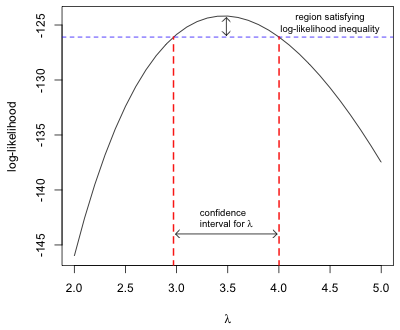
\includegraphics[width=0.7\textwidth]{./figures/proflike_example}
% \caption[External figure]{Caption line below the figure.} % Caption line pasted below puts \includegraphics[]{} the caption below the figure. 
% \label{fig:proflike}
% \end{figure}